\documentclass[justified,a4paper,symmetric,nobib]{tufte-book}

% Packages setup
\input{Preamble/Bibliography_fix}
\input{Preamble/Packages}
\input{Preamble/Formatting}
\input{Preamble/Commands}

% Bibliographt file
\addbibresource{Preamble/References.bib}

% Book metadata
\title{}
\author{Clebson Abati Graeff}
\publisher{Universidade Tecnológica Federal do Paraná\\câmpus Pato Branco}
\newsavebox{\titleimage}
\savebox{\titleimage}{\includegraphics[height=10cm]{Ilustrations/capa.png}}

\title[Notas de Aula de Laboratório A]{%
  Notas de aula: \\ Laboratório de Física A \par \vfill
  \hfill\usebox{\titleimage}}
  
\begin{document}

\frontmatter
\pagestyle{empty}

% Front matter

% r.3 full title page
\maketitlepage

% v.4 copyright page
\newpage
\include{Front_Matter/Copyright_Page}

% calendário
%\include{Front_Matter/Calendar}

% r.5 contents
\setcounter{tocdepth}{2}
\tableofcontents

%\listoffigures
%\listoftables

% r.9 introduction
\cleardoublepage
\include{Chapters/Introduction}


\mainmatter
\pagestyle{fancy}

\part{Medidas, Técnicas de Análise de Dados}

\input{Chapters/Medidas}
\chapter{Gráficos}
\label{Chap:Graficos}

\begin{fullwidth}
{\it
Uma maneira simples de verificar a relação entre duas grandezas é a elaboração de um gráfico de dispersão. Apesar de não podermos verificar valores exatos em um gráfico, uma observação do comportamento geral de um conjunto de pontos pode ser muito esclarecedora, principalmente se levarmos em conta que todas as medidas efetuadas sofrem uma dispersão aleatória em torno de seus valores ideais. Verificaremos como elaborar um gráfico de maneira a evidenciar o comportamento das variáveis consideradas e, no Capítulo~\ref{Chap:RegressoLinear}, verificaremos como descrever de maneira idealizada a dependência entre as variáveis.
}
\end{fullwidth}

%%%%%%%%%%%%%%%%%%
\section{Gráficos}
%%%%%%%%%%%%%%%%%%

Um gráfico é uma maneira de transformar um conjunto de dados numéricos em uma figura, relacionando valores numéricos a escalas de cor, distâncias ou áreas. No livro \emph{The Visual Display of Quantitative Information}\cite{Tufte2001} (\emph{A representação visual de informações quantitativas}, em um tradução livre), Edward R. Tufte
afirma que
\begin{quote}
	Gráficos mostram quantidades visualmente através do uso combinado de pontos, linhas, um sistema de coordenadas, números, símbolos, palavras, sombreamento, e cor.
\end{quote}
%
e que
\begin{quote}
	Gráficos modernos podem fazer muito mais que simplesmente substituir pequenas tabelas de dados. Quando utilizados em seu máximo potencial, gráficos são instrumentos para raciocinar sobre informações quantitativas. Frequentemente a maneira mais efetiva para descrever, explorar, e sumarizar um conjunto de números ---~mesmo um conjunto muito grande~--- é através de figuras de tais números.
\end{quote}

Tufte afirma que talvez em virtude da diversidade de técnicas e informações necessárias ---~habilidades artísticas e matemáticas, dados experimentais~--- a utilização de figuras abstratas para representar números é relativamente recente (1750 em diante). Dentre os autores que desenvolveram o campo da representação gráfica de dados, ele destaca o trabalho de William Playfair, que desenvolveu melhorias para vários tipos de gráficos. Tufte também destaca o trabalho de Johann Heinrich Lambert, que percebe que os gráficos não precisam necessariamente relacionar quantidades em analogia ao mundo físico ---~como séries temporais, isto é, a evolução de um valor qualquer de acordo com a evolução do tempo~---, mas podem ser elaborados para quaisquer duas variáveis cujas relações desejamos verificar:

\begin{quote}
	Temos em geral duas quantidades variáveis, $x$, $y$, que serão comparadas uma à outra por observação, de forma que para cada valor de $x$ ---~que pode ser considerada como uma abscissa~--- determinamos a ordenada correspondente $y$. Se as observações experimentais fossem completamente precisas, essas ordenadas resultariam em um número de pontos através dos quais uma curva ou uma reta deveriam ser traçadas.\cite{Lambert}
\end{quote}

Existem vários tipos de gráficos, cada um com o objetivo de evidenciar características específicas do conjunto de dados em questão:
\begin{itemize}
	\item \emph{Gráficos de setores} servem bem o propósito de mostrar a contribuição relativa de várias parcelas que perfazem um todo;
	\item \emph{Gráficos de colunas/barras} servem para comparação entre diversos valores absolutos;
	\item \emph{Gráficos de colunas/barras empilhadas} denotam valores absolutos e demonstram a composição relativa de várias contribuições para o todo. Une as propriedades dos dois tipos anteriores;
	\item \emph{Séries temporais} denotam a evolução temporal de variáveis com o tempo;
	\item \emph{Mapas de dados} servem para demonstrar dados que variam de acordo com a distribuição geográfica;
	\item \emph{Gráficos de dispersão} permitem verificar a relação entre duas variáveis quaisquer;
	\item \emph{Histogramas} são similares aos gráficos de barra, mas voltados à apresentação de contagens de eventos em diversos intervalos.
	%\item \emph{Gráficos de radar}
	%\item \emph{Gráficos de curva de nível}
\end{itemize}
%
Em comum a todos os tipos de gráfico está a utilização de dimensões como área e comprimento, ou tonalidades de cor, para representar informações numéricas.

Temos especial interesse nos gráficos de dispersão. Esse tipo de gráfico serve para verificar relações de causa e efeito entre duas variáveis quaisquer. De acordo com Tufte,
\begin{quote}
	[...] Na literatura científica moderna, em torno de 40\% dos gráficos publicados têm uma forma relacional, com duas ou mais variáveis. Isto não é sem propósito, já que os gráficos relacionais ---~em sua forma mais simples, o gráfico de dispersão e suas variantes~--- é o mais formidável de todos os tipos de gráficos. Eles ligam pelo menos duas variáveis, encorajando e mesmo suplicando que o leitor se pergunte qual é a possível relação causal entre elas. Eles confrontam as teorias causais [...] com evidências empíricas.
\end{quote}
%
De fato, estamos interessados em verificar experimentalmente a relação entre diversas variáveis através de experimentos. Além disso, desejamos testar teorias científicas, procurando confirmar ou refutar suas validades.

Finalmente, como recomendações gerais para a elaboração de gráficos, Tufte destaca:
\begin{itemize}
	\item \emph{A representação de números através de medidas de superfície em um gráfico deve ser proporcional às quantidades numéricas representadas}.\footnote[][-3cm]{Esse item é bastante visível ao se analisar um gráfico de campanha política: o candidato que deseja evidenciar sua vantagem costuma realizar um corte de forma que o zero não seja no menor valor da escala mostrada e também adota uma largura maior para sua coluna. Dessa forma uma diferença insignificante (menor que o erro da própria pesquisa) parece muito grande.}
	\item \emph{Cada parte de um gráfico gera expectativa visual sobre as outras partes. Se uma escala que se move em intervalos regulares, por exemplo, se espera que ela continue a fazê-lo. Mostre a variação dos dados, não variação na elaboração do gráfico.}
	\item \emph{Em séries temporais, ao se mostrar dados relativos a dinheiro, geralmente é melhor utilizar quantidades corrigidas pela inflação}.
	\item \emph{O número de dimensões utilizadas para demonstrar informações não deve exceder o número de dimensões dos dados}\footnote{As dimensões são as maneiras diferentes que os dados podem variar. Se, por exemplo, desejamos comparar o número de habitantes de diversas cidades, devemos utilizar uma figura com uma dimensão (um gráfico de barras) e não com duas (a área de um círculo).}.
	\item \emph{Acima de tudo, mostre os dados.}\footnote{Isto é, faça um gráfico simples, sem floreios, que mostre os dados.}
\end{itemize}


%%%%%%%%%%%%%%%%%%%%%%%%%%%%%%%%%%
\section{Gráficos de dispersão}
%%%%%%%%%%%%%%%%%%%%%%%%%%%%%%%%%%

Gráficos de dispersão são ferramentas muito usadas para visualizar relações matemáticas entre uma função e seu argumento. Por exemplo, denominamos a função $f(x) = A + Bx$ como ``equação da reta'', pois seu gráfico é uma reta. Cada função tem um gráfico característico. 

Em experimentos de laboratório é comum procuramos estabelecer a relação entre duas grandezas. Uma delas variamos arbitrariamente e denominamos como \emph{variável independente}, já a outra medimos e ---~como seus valores variam em resposta aos da variável independente~--- a denominamos como \emph{variável dependente}. Tais variáveis são representadas nos eixo $x$  (abscissas) e $y$ (ordenadas), respectivamente, sendo o primeiro o eixo horizontal e o segundo o vertical. É comum nos referirmos a um gráfico como sendo do tipo $\Delta x \times t$, $\Delta L \times \Delta T$, etc. ---~ou ainda $\Delta x \;vs\; t$, $\Delta L \;vs\; \Delta T$, etc.~---. Nessa notação, a variável à esquerda do símbolo $\times$, ou do $vs$ (\emph{versus}), denota a quantidade que corresponde ao eixo vertical, enquanto o símbolo à direita denota a variável que corresponde ao eixo horizontal.

O maior objetivo de uma teoria é justamente encontrar a relação matemática $f$ que relaciona $x$ e $y$, ou seja, que nos dá $y$ \emph{em função de} $x$: $y = f(x)$. Isso não é algo que possa ser retirado dos gráficos de uma maneira simples, por diversas razões. Primeiramente, os dados experimentais se distribuem em torno do comportamento ideal devido a variações aleatórias. Além disso, mesmo que possamos tirar uma conclusão a partir do gráfico, tal conclusão só é válida para o intervalo de valores que compreende as medidas, podendo ser diferente em outras regiões. Finalmente, uma relação extraída dos dados experimentais não consegue explicar em argumentos lógicos o mecanismo que relaciona uma variável à outra, portanto não explicando o comportamento. De qualquer forma, uma gráfico que mostra uma dependência confiável de uma variável em relação a outra já abre um caminho para a investigação.

Também podemos utilizar os dados experimentais para \emph{verificar a validade de previsões teóricas}. Nesse caso podemos empregar gráficos como meio de evidenciar as concordâncias e discrepâncias entre a previsão teórica de os dados experimentais. Em geral, as previsões teóricas são representadas visualmente por \emph{curvas contínuas}, enquanto os dados experimentais são representados por \emph{pontos}. Essa distinção reflete o fato de que as previsões teóricas relacionam as variáveis para todos os valores que elas podem assumir dentro de um intervalo; já para os dados experimentais as informações são obtidas para valores particulares das variáveis.

%%%%%%%%%%%%%%%%%%%%%%%%%%%%%%%%%%%%%%%%%%%%%%%%%%%%%%%%%%%%%%%
\subsection{Principais elementos de um gráfico de dispersão}
%%%%%%%%%%%%%%%%%%%%%%%%%%%%%%%%%%%%%%%%%%%%%%%%%%%%%%%%%%%%%%%

\begin{marginfigure}[5cm]
\centering
\begin{tikzpicture}[>=Stealth, extended line/.style={shorten >=-#1,shorten <=-#1},
 extended line/.default=3mm]] % talvez fosse melhor amplicar com scale=1.5
    % Draw axes: acho que o |- é pra desenhar um "canto", um L
    \draw [<->,thick] (-0.2,3) node (yaxis) [below left] {$T$ $\tcdegree$C}
        |- (3.5,0) node (xaxis) [below] {$t$ (s)};
        
    % Desenhar função: (estamos usando a eq. para fazer o desenho no papel milimetrado para 
    % ajustar o eixo y; o eixo x está sendo ajustado para que o domain reflita o intervalo
    % da variável para os dados experimentais)  
    \draw[smooth, densely dashed, name path=plotb,samples=1000,domain=0:3.0]
    plot(\x,{(82.6984623879127 * exp(-0.00310112376447134*\x*300/3.0) - 30) * 3/(95 - 30)});
    
    % escala do eixo x
    \draw(0,0) -- (0,-0.1) node[below]{\footnotesize{0}};
    %\draw(0.5,0) -- (0.5,-0.1) node[below]{\footnotesize{50}};
    \draw(1,0) -- (1,-0.1) node[below]{\footnotesize{100}};
    %\draw(1.5,0) -- (1.5,-0.1) node[below]{\footnotesize{150}};
    \draw(2,0) -- (2,-0.1) node[below]{\footnotesize{200}};
    %\draw(2.5,0) -- (2.5,-0.1) node[below]{\footnotesize{250}};
    \draw(3,0) -- (3,-0.1) node[below]{\footnotesize{300}};
    
    % escala do eixo y
    \draw(-0.2,0.46154) -- (-0.3,0.46154) node[left]{\footnotesize{40}};
    \draw(-0.2,1.3846) -- (-0.3,1.3846) node[left]{\footnotesize{60}};
    \draw(-0.2,2.3077) -- (-0.3,2.3077) node[left]{\footnotesize{80}};
    
    % pontos
    \fill (0.3107,2.1692) circle (1.5pt);
    \fill (0.6778,1.7077) circle (1.5pt);
    \fill (1.1526,1.2462) circle (1.5pt);
    \fill (1.7032,0.7846) circle (1.5pt);
    \fill (2.6804,0.3231) circle (1.5pt);
    
     
\end{tikzpicture}
\caption{Elementos fundamentais de um gráfico.}
\end{marginfigure}

Os elementos mais notáveis de um gráfico de dispersão são:
\begin{description}
	\item[Eixos:] Os valores das variáveis dependente e independente  são expressos pelas distâncias ao longo dos eixos vertical e horizontal em relação à origem (encontro dos dois eixos). Muitas vezes os valores das variáveis são distantes de zero e não podem ser verificados adequadamente se um dos eixos ---~ou mesmo ambos~--- iniciarem em zero. Por isso, é comum que se realizem ``cortes'' nos eixos de maneira que eles iniciem em valores convenientes. Nesse caso, os valores são expressados por meio da distância relativa que os pontos ocupam entre duas marcas numeradas nos eixos (veja o item seguinte). Os eixos devem ser nomeados com a variável que está sendo representada e suas unidades.
	\item[Escalas:] Para que a leitura do gráfico possa ser efetuada de uma maneira quantitativa, ainda que aproximada, é importante que se efetuem marcas nos eixos e que elas sejam numeradas com os valores que elas representam no eixo. Tais marcas não precisam iniciar em zero, e nem mesmo precisam necessariamente estarem posicionadas na origem, porém devem ser efetuadas em intervalos regulares e com números de fácil leitura. Nas escalas não devem ser marcados os valores das abscissas e ordenadas dos pontos.\footnote{Exceto no caso em que os próprios valores das variáveis ocorrem em intervalos regulares e tais intervalos correspondem ao mais adequado para a escala do eixo. Isso ocorre mais comumente com os valores do eixo independente (horizontal).}
	\item[Pontos experimentais:] Os dados experimentais são representados através de pontos na área retangular delimitada pelos eixos horizontal e vertical. A localização dos pontos é aquela do encontro das retas paralelas aos eixos horizontal e vertical e que passam pelas posições desses eixos que correspondem aos valores que desejamos representar. Para que o ponto seja facilmente visível, indica-se a utilização de quadrados, círculos, triângulos, etc. centrados no ponto de encontro das retas. Caso mais que um conjunto de dados seja representado no mesmo gráfico, devem ser utilizados símbolos diferentes para cada conjunto.
\end{description}

\noindent{}Como elementos opcionais, temos:
\begin{description}
	\item[Legenda:] Se temos somente um conjunto de dados, a legenda pode ser dispensada. No entanto, se temos dois ou mais conjuntos ---~ou mesmo curvas~---, representados no mesmo gráfico, é essencial que seja feita uma legenda indicando o que cada símbolo representa.
	\item[Linha de tendência:] Uma reta ou curva que represente o comportamento ``médio'' dos pontos é denominada como \emph{linha de tendência}. Muitas vezes estaremos interessados nesse tipo de curva, porém verificaremos como calculá-las adequadamente no Capítulo~\ref{Chap:RegressoLinear}. Tal curva deve ficar restrita à área do gráfico que contém os dados experimentais (entre os valores mínimo $x_{min}$ e máximo $x_{max}$ para as abscissas dos dados experimentais).
	\item[Título:] Um título pode ser adicionado ao gráfico indicando como eles foram obtidos. Um exemplo de título adequado é ``Valores do deslocamento de um corpo em queda livre em função do tempo''; Uma versão inadequada desse título seria ``Gráfico de $\Delta x$ em função de $t$''.
\end{description}
%
Muitas vezes alguns desses elementos são omitidos. O título e a legenda, por exemplo, podem ser descritos na \emph{legenda da figura} ---~o pequeno texto que aparece abaixo das figuras, como na Figura~\ref{Fig:GraficoResfriamento}~---. Já a linha de tendência pode ser omitida por não ser de interesse do autor do gráfico.

%%%%%%%%%%%%%%%%%%%%%%%%%%%%%%%%%%%%%%%%%%%%%%%%%%
\paragraph{Exemplo de um gráfico de dispersão}
%%%%%%%%%%%%%%%%%%%%%%%%%%%%%%%%%%%%%%%%%%%%%%%%%%

\begin{margintable}[-3cm]
\centering
\begin{tabular}{ccccc}
\toprule
\multicolumn{2}{c}{Tubo 1} && \multicolumn{2}{c}{Tubo 2} \\
\cmidrule{1-2}\cmidrule{4-5}
$t$~(s) & $T~\tcdegree\textrm{C}$ & & $t$~(s) & $T~\tcdegree\textrm{C}$ \\
\midrule
\np{0}		& \np{98}	&& \np{0}		& \np{92} \\ 
\np{5,71}	& \np{93}	&& \np{8,27} 	& \np{87} \\
\np{17,79}	& \np{88}	&& \np{17,43}	& \np{82} \\
\np{34,50}	& \np{83}	&& \np{31,07}	& \np{77} \\
\np{61,63}	& \np{78}	&& \np{44,98}	& \np{72} \\
\np{83,96}	& \np{73}	&& \np{67,78}	& \np{67} \\
\np{109,09}	& \np{68}	&& \np{96,57}	& \np{62} \\
\np{130,78}	& \np{63}	&& \np{115,26}	& \np{57} \\
\np{149,09}	& \np{58}	&& \np{135,78}	& \np{52} \\
\np{184,21}	& \np{53}	&& \np{170,32}	& \np{47} \\
\np{217,09}	& \np{48}	&& \np{213,28}	& \np{42} \\
\np{261,28}	& \np{43}	&& \np{268,04}	& \np{37} \\
\np{315,90}	& \np{38}	&& \np{349,44}	& \np{32} \\
\np{373,35}	& \np{33}	&& \np{465,71}	& \np{27} \\
\np{470,55}	& \np{28}	&& \np{575,21}	& \np{24} \\
\np{504,21}	& \np{25} \\
\bottomrule
\end{tabular}
\vspace{1mm}
\caption{Dados para a temperatura de tubos metálicos em função do tempo para o processo de resfriamento convectivo.\label{Tab:TabelaDadosResfriamento}}
\end{margintable}

Se tomarmos as medidas da Tabela~\ref{Tab:TabelaDadosResfriamento}, podemos fazer um gráfico como o da Figura~\ref{Fig:GraficoResfriamento}. Nesse gráfico podemos perceber que foram aplicados alguns princípios básicos para a elaboração de um gráfico adequado:
\begin{itemize}
	\item O gráfico deve ter os dois eixos com numerações que aparecem em \emph{intervalos regulares} ---~a cada 100 no eixo $x$ e a cada 10 no eixo $y$~---.
	\item O eixo $y$ foi ``cortado'', iniciando em 20. Isto é adequado pois não existem dados cujos valores da variável dependente sejam menores que 20.
	
\begin{figure*}[!htb]
\centering
\caption{Gráfico dos dados da Tabela~\ref{Tab:TabelaDadosResfriamento}.\label{Fig:GraficoResfriamento}}
\input{Graphics/Features/features.tex}
\end{figure*}

	\item Os eixos começam e terminam em valores que permitem que toda a área disponível do gráfico seja bem utilizada.
	\item O gráfico possui uma legenda indicando o que os pontos representam.
	\item Os eixos foram nomeados e indicam as unidades dos dados.
	\item O título descreve sucintamente o que o gráfico representa.
\end{itemize}

\noindent{}Note ainda que o gráfico possui um eixo acima e outro à direita, formando um retângulo. Essa é uma opção muito utilizada ao elaborarmos um gráfico utilizando um computador. Na Seção~\ref{Sec:SoftwareGraficos} discutiremos o emprego desse tipo de ferramenta, tornando a elaboração de gráficos uma tarefa rápida e eficiente.

%%%%%%%%%%%%%%%%%%%%%%%%%%%%%%%%%%%%%%%%%%%%%%%%%%%%%%%%%%%
\subsection{Problemas mais comuns em gráficos de dispersão}
%%%%%%%%%%%%%%%%%%%%%%%%%%%%%%%%%%%%%%%%%%%%%%%%%%%%%%%%%%%

A elaboração de um gráfico não é uma tarefa que podemos reduzir a um certo número de passos. Um gráfico deve ser utilizado de maneira a evidenciar dados ou seu comportamento e muitas vezes isso implica em fugirmos das regras mais comuns: por exemplo, se desejamos mostrar com o auxílio de uma linha de tendência qual é o valor estimado da variável dependente em uma região do gráfico distante dos pontos experimentais, inevitavelmente vamos precisar estender os eixos de forma a incluir a região desejada. Ainda assim, podemos recomendar que os seguintes itens sejam evitados:
\begin{description}
	\item[Não utilizar adequadamente a área do gráfico:] Muitas vezes nossos dados não iniciam em zero. Nesse caso devemos escolher um número próximo, porém inferior, ao primeiro valor que ocorre naquele eixo e iniciar o eixo em tal número. Se, por exemplo, devemos marcar em um eixo os valores \np{107,25}, \np{115,12}, \np{129,90}, \np{138,22}, etc., uma boa escolha é iniciar o eixo em 100 e realizarmos as marcações no eixo a cada 10. Outra escolha adequada seria iniciar o eixo em 105 ---~porém, nesse caso, não marcamos o ``canto'' do gráfico como 105~---. Realizamos a marcação em 110 e daí em diante a cada 10.
	\item[Não utilizar espaçamento regular na numeração dos eixos:] Marcações irregulares, isto é, com ``espaçamento variável'' não devem ser realizadas. Utilizando os dados do item acima, poderíamos realizar marcações no eixo em \np{105}, \np{115}, \np{130} e \np{140}. Porém a distância entre essas marcações não é regular, o que dificulta a leitura do gráfico.
	\item[Marcar os valores de $x$ e $y$ dos pontos experimentais:] Os valores de abscissas e de ordenadas dos pontos não devem aparecer nos eixos ordenados (exceto se elas coincidem com os valores regulares escolhidos para rotular a escala). Veja que no gráfico da Figura~\ref{Fig:GraficoResfriamento} ocorrem muitos valores que ficam entre duas marcações quaisquer, porém os valores correspondentes aos pontos não devem ser marcados no eixo.
	\item[Linhas que ligam os pontos aos eixos:] Muitos alunos traçam linhas para auxiliar a marcação dos pontos experimentais, mas não as apagam após marcá-lo. Tais linhas não têm propósito uma vez que o ponto já tenha sido marcado e acabam dificultando a visualização dos dados experimentais. Caso queiramos saber exatamente os valores das variáveis independente e dependente, podemos verificá-los na tabela de dados.
	\item[Linhas que ligam os pontos entre si:] Os pontos marcados a partir de dados experimentais nunca devem ser ligados entre si. Quando marcamos curvas ou retas em um gráfico, isso significa que temos conhecimento sobre todos os pontos que compõe aquela curva. Isso só pode ser razoável para curvas que denotam previsões teóricas, não para dados experimentais. Estes são verificados ``pontualmente'' e não podemos afirmar nada sobre o que obteríamos entre dois pontos quaisquer. Portanto, a reta que liga dois pontos experimentais não carrega informação alguma e não deve ser traçada. Veja a Figura~\ref{GraficoErrado} para um exemplo do que não fazer.
\end{description}

\begin{figure*}
\centering
\forcerectofloat
\input{Graphics/Certo_Errado/errado}
\caption{\textbf{Exemplo do que não fazer}: ligar os pontos experimentais, não nomear os eixos, não colocar unidades.}
\label{GraficoErrado}
\end{figure*}

%\begin{figure*}
%\centering
%\forcerectofloat
%\label{ExemploGrafico}
%\input{Graphics/Certo_Errado/graph_dois_conjuntos}
%\caption{Exemplo de gráfico contendo vários conjuntos de dados. Notem que cada conjunto usa um símbolo diferente para os dados e que não ligamos os pontos. Além disso, fazemos um corte no eixo $x$ para aproveitar a área do gráfico.}
%\end{figure*}

%%%%%%%%%%%%%%%%%%%%%%%%%%%%%%%%%%%%%%%%%%%%%%%%%%%%%%%%
\subsection{Elaborando um gráfico com papel milimetrado}
%%%%%%%%%%%%%%%%%%%%%%%%%%%%%%%%%%%%%%%%%%%%%%%%%%%%%%%%

Hoje podemos fazer um gráfico rapidamente usando um programa de computador. No entanto, é interessante fazer alguns gráficos com papel milimetrado e lápis/caneta para sabermos o que tais programas estão fazendo.

Elaborar um gráfico em papel milimetrado é uma questão de observar as regras gerais para a elaboração de gráficos e usar regras de três. O procedimento para elaborar o gráfico consiste no seguinte (veja a Figura~\ref{Fig:EsquemaElabGrafPapelMil}):
\begin{enumerate}
	\item Verificar quais os valores mínimo $x_i$ e máximo $x_f$ para o eixo $x$. Tais valores devem ser um pouco menor e um pouco maior que os valores mínimo e máximo para as abscissas dos dados experimentais, respectivamente.
	\item Verificar quais os valores mínimo $y_i$ e máximo $y_f$ para o eixo $y$. Como no cado do eixo $x$, os valores escolhidos devem ser um pouco menor e um pouco maior que os valores das ordenadas dos pontos experimentais, respectivamente.
	\item Verificar o tamanho do papel e desenhar os eixos \emph{dentro da área milimetrada} e não na borda dessa área. Em geral, deixa-se um centímetro entre a borda da área milimetrada e o eixo para que possamos fazer as escalas. Com isso determinamos as medidas $m_x$ e $m_y$ dos eixos horizontal e vertical no papel.
	
\begin{marginfigure}[-4cm]
    \begin{tikzpicture}[>=Stealth]
	    \draw[->] (0,0) -- (0,2.5) node[left]{$y$};
	    \draw[->] (0,0) -- (4.3,0) node[below]{$x$};
	    \draw (0,0) -- (0,-0.1) node[below]{0};
	    \draw (4,0) -- (4,-0.1) node[below]{$x_f$};
	    \draw[|-|] (0,-0.6) -- node[below]{$m_x$} (4,-0.6);
	    
	    \draw (2,0.5) circle[radius=0.1];
	    \draw[fill] (2,0.5) circle[radius=0.01];
	    \draw[<->] (0,0.8) -- node[above]{$d_x$} (2,0.8);
	    \draw[dotted] (2,0) -- (2,1);
    \end{tikzpicture}
	\caption{Variáveis para o cálculo da posição de um ponto em um gráfico em que o eixo $x$ inicia em zero.}
	\label{Fig:VarGraphInicioZero}
\end{marginfigure}

	\item Se escolhermos $x_i = 0$, temos que a distância $m_x$ em relação à origem do eixo $x$ representa o valor $x_f$ que escolhemos para o final do eixo\footnote{O raciocínio para o eixo $y$ é o mesmo, por isso mostramos somente para o eixo $x$.}. Isso é equivalente a dizer que cada unidade de medida no eixo $x$ equivale a uma quantidade\footnote{O que temos é uma regra de \emph{proporção}, ou seja, uma regra de três: \begin{align} d &\quad\text{\textemdash}\quad x_p \\ m &\quad\text{\textemdash}\quad x_f, \end{align} o que resulta em \begin{equation} d_x = x_p \frac{m_x}{x_f}. \end{equation}}
	\begin{equation}
		f_x = \frac{x_f}{m}.
	\end{equation}
	Assim, se precisamos representar um valor $x_p$ de um ponto $P = (x_p,y_p)$ qualquer, calculamos a distância $d_x$ em relação à origem ---~veja a Figura~\ref{Fig:VarGraphInicioZero}~---através de\footnote{Note que a fração que aparece nessa equação é um valor constante. Calculando tal valor podemos simplesmente multiplicá-lo pelo valor $x_p$ de cada ponto para descobrir quanto cada um dista da origem.}
	\begin{equation}
		d_x = \frac{x_p}{f_x} = x_p \frac{m_x}{x_f}.
	\end{equation}

	Se fizermos um corte no eixo $x$ em um valor $x_i$, temos que uma unidade de medida nesse eixo representa uma quantidade (veja a Figura~\ref{Fig:EsquemaElabGrafPapelMil})
	\begin{equation}
		f_x = \frac{x_f-x_i}{m_x}.
	\end{equation}
	Dessa forma, se precisamos representar um valor $x_p$, devemos dividir pelo fator $f_x$ somente o valor que \emph{excede} o valor do corte $x_i$. Portanto, a distância $d_x$ é dada por\footnote{Veja que se tivermos um ponto em que $x_p$ é igual a $x_i$, ele deve ficar sobre a posição de corte do eixo ($d_x = 0$), o que está de acordo com o que a equação prevê. Note também que novamente o valor da fração é constante, facilitando o cálculo da distância.},
	\begin{equation}\label{Eq:DistDX}
		d_x = \frac{(x_p-x_i)}{f_x} = (x_p-x_i)\frac{m_x}{x_f-x_i}.
	\end{equation}
	
	Vamos considerar, por exemplo, um conjunto de dados cujas abscissas correspondem a uma variável $t$, cujas unidades são segundos. Verificamos que o menor valor de abscissa para os pontos é \np[s]{36,29} e o maior \np[s]{104,04}. Todas as abscissas estão compreendidas entre \np[s]{30} e \np[s]{110} e podemos escolher tais valores\footnote[][-1cm]{Outra escolha possível seria entre \np[s]{35} e \np[s]{105}. No entanto, devemos tomar cuidado com a escolha pois alguns pontos podem ficar muito próximos dos eixos, dificultando a leitura do gráfico.} como o início e o fim do eixo $x$. A medida do eixo no gráfico é $m_x = \np[cm]{25,00}$. Assim, se desejamos encontrar a distância $d_x$ a partir do início do eixo em que devemos marcar um ponto cuja abscissa é $x_p=\np[s]{47,20}$ temos
	\begin{align}
		d_x &= (\np{47,20} - 30)\frac{25,00}{110 - 30} \\
		  &= \numprint[cm]{5,375}.
	\end{align}
	\item Podemos determinar a posição do ponto $P = (x_p,y_p)$ no eixo $y$ de maneira análoga, calculando a distância $d_y$ através de
		\begin{equation}\label{Eq:DistDY}
			d_y = (y_p-y_i)\frac{m_y}{y_f-y_i}.
		\end{equation}
	\item Também podemos calcular a posição de uma marca das escalas dos eixos $x$ e $y$ utilizando as Equações~\eqref{Eq:DistDX} e~\eqref{Eq:DistDY}. Para isso basta utilizarmos o valor que desejamos marcar no lugar da abscissa $x_p$ ou da ordenada $y_p$. Após encontrarmos a posição das duas primeiras marcas, no entanto, basta verificar a distância entre elas e utilizá-la para marcar a posição das demais marcas, já que o espaçamento deve ser constante.
\end{enumerate}

\begin{figure*}
\begin{tikzpicture}[>=Stealth]

	% Área milimetrada
	\draw (0.25,0.5) rectangle (16.5,10);
	\draw[step=.25cm, gray, densely dotted] (0.25,0.5) grid (16.5,10);
	
	% Eixos
	\draw[->, thick] (1.5,1.4) node[anchor=north]{$x_i$} -- (1.5,9.5) node[anchor=east,gray] {$y$ (Un)};
	\draw[->, thick] (1.4,1.5) node[left]{$y_i$} -- (15.5,1.5);
	\node[gray] (x) at (15.8,1.2) {$x$ (Un)};

	% tics finais
	\draw[thick] (15,1.5) -- (15,1.4) node[anchor=north]{$x_f$};
	\draw[thick] (1.5, 9) -- (1.4, 9) node[anchor=east]{$y_f$};
	
	% Tamanho do eixo $x$
	\draw (1.5,0.875) -- (7.9,0.875);
	\draw (8.6,0.875) -- (15,0.875);
	\draw (1.5,0.75) -- (1.5,1);
	\draw (15,0.75) -- (15,1);
	\draw (8.25,0.875) node{$m_x$};
	
	% Tamanho do eixo $y$
	\draw (0.625,1.5) -- (0.625,5);
	\draw (0.625,5.5) -- (0.625,9);
	\draw (0.5,1.5) -- (0.75,1.5);
	\draw (0.5, 9) -- (0.75,9);
	\draw (0.625, 5.25) node{$m_y$};
	
	% Ponto experimental
	\draw[thick] (6.6,5.1) circle (0.1cm) node[anchor=south west]{$P = (x_p,y_p)$};
	\draw[fill=black] (6.6,5.1) circle (0.1mm);
	
	% Distância do ponto ao eixo $x$
	\draw (1.5,5.5) -- node[anchor=south, above=1mm]{$d_x$} (6.6,5.5);
	\draw (6.6,5.6) -- (6.6,5.4);
	
	% Distância do ponto ao eixo $y$
	\draw (7,1.5) -- node[anchor=west, right=1mm]{$d_y$} (7,5.1);
	\draw (6.9,5.1) -- (7.1,5.1);
	
	% Limites da região dos pontos
	\draw[dashed] (1.5,9) -- (15,9) -- (15,1.5);
	
	% Título do gráfico
	\draw[gray] (8.25,9.5) node{\Large{Título do gráfico}};

\end{tikzpicture}
\caption{Esquema para a elaboração de um gráfico em papel milimetrado.\label{Fig:EsquemaElabGrafPapelMil}}
\end{figure*}

Utilizando o procedimento acima, todos os pontos experimentais estarão distribuídos dentro da área demarcada pelo valor máximo $y_f$ no eixo $y$ e pelo valor máximo $x_f$ no eixo $x$ ---~ na Figura~\ref{Fig:EsquemaElabGrafPapelMil}, a região retangular delimitada pelos eixos $x$ e $y$, e pelas retas tracejadas~---. Veja que o adequado aproveitamento dessa região está diretamente ligado aos valores escolhidos para $x_i$, $y_i$, $x_f$ e $y_f$: se, por exemplo, escolhermos valores para $x_i$ e $y_i$ que não sejam menores que os valores mínimos das abscissas e ordenadas dos pontos, teremos pontos abaixo do eixo $x$, à esquerda do eixo $y$, ou ambos. Outro problema, nesse caso, é que os pontos podem ficar sobre os eixos ou muito próximos deles, dificultando a sua visualização. Por outro lado, se escolhermos valores para $x_i$ e $y_i$ muito menores que os valores mínimos das abscissas e ordenadas dos pontos, teremos grandes regiões vazias à esquerda e/ou abaixo dos pontos do gráfico. Analogamente, devemos escolher valores de $x_f$ e $y_f$ que sejam maiores que os valores máximos das abscissas e ordenadas dos pontos, porém não muito maiores: se escolhermos valores menores que os máximos, teremos pontos fora do gráfico (à direita/acima das retas tracejadas); se escolhermos valores muito maiores que os máximos, teremos regiões vazias à direta e/ou acima dos pontos experimentais. 

Uma dificuldade prática dos cálculos acima é a de que muitas vezes eles incorrem em fatores de escala não muito práticos, pois resultam em números ``quebrados'' que tornam a marcação dos pontos no papel milimetrado suscetível a erros. Uma maneira de contornar esse problema é aproximarmos a escala: tomando o eixo $x$, por exemplo, calculamos através dos valores $x_f$, $x_i$ e $m_x$ um fator de escala $f_x$ onde
		\begin{equation}
			f_x = \frac{x_f - x_i}{m_x}.
		\end{equation}
Após calculá-lo, o arredondamos para algum dos valores seguintes: 1, 2, 2,5, 4, 5 ou 10, ou qualquer múltiplo ou submúltiplo decimal desses (isto é, esses números multiplicados por 10 elevado a alguma potência inteira), sempre fazendo o arredondamento para cima. A partir desse valor arredondado $f'_x$, podemos calcular a distância $d_x$ entre o início do eixo e o ponto através de
		\begin{equation}
			d_x = \frac{x_p - x_i}{f'_x}.
		\end{equation}

%%%%%%%%%%%%%%%%%%% Futuro
%\paragraph{Exemplo}
%%%%%%%%%%%%%%%%%%%
%\comment{Colocar exemplo aqui}

%%%%%%%%%%%%%%%%%%%%%%%%%%%%%%%%%%%%%%%%%%%%%%%%%%%%%%%%%%%%%%
\section{Elaborando um gráfico com o auxílio de um computador}
\label{Sec:SoftwareGraficos}
%%%%%%%%%%%%%%%%%%%%%%%%%%%%%%%%%%%%%%%%%%%%%%%%%%%%%%%%%%%%%%

Mesmo para um número reduzido de pontos, a elaboração de um gráfico em papel milimetrado é uma tarefa que toma um tempo razoável. Com a onipresença de ferramentas computacionais, no entanto, podemos realizar esse trabalho de uma maneira muito mais eficiente.

É claro que cada programa tem suas características particulares e, dada a profusão de alternativas que suportam a elaboração de gráficos, explicar o funcionamento de cada um deles seria inútil. De qualquer forma, todos suportam mais ou menos as mesmas funções. Cabe, no entanto, fazer uma diferenciação quanto à proposta dos mais utilizados:
\begin{description}
    \item[Software de planilhas:] Talvez a primeira opção para a elaboração rápida de um gráfico, os softwares de planilha como o \emph{Microsoft Excel} e o \emph{LibreOffice Calc} (gratuito) oferecem diversos tipos de gráficos. Para criar um gráfico, basta listar os dados em duas colunas, sendo a primeira a das abscissas e a segunda das ordenadas, sendo que cada linha corresponde a um par ordenado (um ponto). Selecionando os dados, basta acionar a função de elaboração de um gráfico e seguir os passos do assistente. Cabe lembrar que devemos selecionar como tipo o `gráfico de dispersão'. Note que essas alternativas costumam não gerar resultados de alta qualidade, mas que com os devidos ajustes podemos considerar satisfatórios;\footnote[][-4cm]{O problema mais recorrente de ambos ao elaborar um gráfico é a escolha automática inadequada de escalas e cortes para os eixos. Apesar de os cortes poderem ser configurados, as marcações necessariamente devem começar na origem, o que pode comprometer um pouco a escolha dos cortes/escalas.}
    \item[Software especializado:] Dentre os programas produzidos especificamente para fins de elaboração de gráficos, cabe mencionar\footnote[][-1cm]{O critério de escolha aqui é `programas que eu uso/lembro que existe'. Certamente existem diversas opções que seriam adequadas.} o \emph{OriginPro}, o \emph{gnuplot} (gratuito), e o \emph{SciDavis} (gratuito). Eles oferecem variados níveis de funcionalidades, porém têm em comum uma maior flexibilidade para a elaboração de gráficos e também funções para a análise de dados, se comparados com os softwares de planinha.
\end{description}

    Os gráficos mostrados nesse capítulo, como a Figura~\ref{Fig:GraficoResfriamento}, foram elaborados usando o \emph{gnuplot}, porém este é um software controlado ou em modo `linha de comando', ou não-interativo (através de \emph{scripts}). Já o \emph{OriginPro} é muito versátil, porém é comercial e as nossas necessidades não justificam a utilização dele. Resta utilizarmos o \emph{SciDavis}, que é bastante adequados às nossas necessidades.
    
%%%%%%%%%%%%%%%%%%%%%%%%%%%%%%%%%%%%%%%%%%%%%%%%%%%%
\subsection{Elaborando um gráfico usando o SciDavis}
%%%%%%%%%%%%%%%%%%%%%%%%%%%%%%%%%%%%%%%%%%%%%%%%%%%%

Vamos verificar abaixo os passos necessários para produzir um gráfico similar ao mostrado na Figura~\ref{Fig:GraficoResfriamento} usando os dados da Tabela~\ref{Tab:TabelaDadosResfriamento} e o \emph{SciDavis}. Apresentaremos abaixo o procedimento para a elaboração de um gráfico com somente um conjunto de dados, um gráfico com conjuntos de dados independentes (que é o caso que buscamos reproduzir), e então um gráfico com conjuntos de dados em que as abscissas são comuns a todos eles.

%%%%%%%%%%%%%%%%%%%%%%%%%%%%%%%%%%%%%%%%%%%%%%%%%%%%%%%
\paragraph{Fazendo gráficos para um conjunto de dados:}
%%%%%%%%%%%%%%%%%%%%%%%%%%%%%%%%%%%%%%%%%%%%%%%%%%%%%%%

Para elaborar um gráfico a partir de dados experimentais, devemos seguir os passos abaixo:
\begin{enumerate}
    \item Imediatamente após abrirmos o software, haverá uma tabela vazia. Sempre que necessário, podemos criar uma nova tabela usando `\textsf{File > New > New table (Ctrl + T)}';
    \item Realize a entrada de dados na tabela. Alternativamente, se os dados estiverem disponíveis em um arquivo CSV ou TSV, podemos realizar a importação dos dados;\footnote{Ao importar os dados, tome cuidado para desmarcar a opção `\textsf{Use first row to name columns}' se a primeira linha contiver dados experimentais e não os nomes das variáveis das colunas.}
    \item Para gerar um gráfico, basta selecionar os dados e selecionar `\textsf{Plot > Scatter}' no menu principal ou no menu de contexto (ativado ao clicar com o botão direito nos dados). Note que após elaborar o gráfico, sempre que ele estiver selecionado, a opção `\textsf{Plot}' no menu principal muda para `\textsf{Graph}' e exibe opções de edição do gráfico. Tal menu pode ser usado para alterar o gráfico, adicionando outras curvas de dados, por exemplo;
    \item Com o gráfico selecionado, aparece um novo menu chamado `\textsf{Format}'. Nele temos diversas opções de modificação:
        \begin{itemize}
            \item Podemos usar `\textsf{Format > Title}' para mudar o título do gráfico;
            \item Em `\textsf{Format > Axis}' podemos escolher quais eixos devem ser mostrados. Por padrão somente o esquerdo e o inferior são mostrados. Se selecionarmos o direto e o superior e marcarmos a opção `\textsf{Show} ', eles serão mostrados. Podemos ocultar a numeração das escalas desmarcando `\textsf{Show Labels}'. Notem que também podemos mudar os nomes de cada um dos quatro eixos, bem como optar por mostrar as marcas dos eixos internamente ou externamente;
            \item Em `\textsf{Format > Scale}' podemos:
                \begin{itemize}
                    \item alterar os pontos de corte de cada um dos eixos (eixos opostos automaticamente terão os mesmos limites);
                    \item escolher o passo (`\textsf{Step} ') das marcas numeradas (`\textsf{Major Ticks}', marcas maiores) da escala, ou quantas marcas devem ser numeradas.\footnote{Note que nem todo valor escolhido funciona pois o software tenta evitar escolhas ruins.} Eixos opostos automaticamente terão as mesmas marcas numeradas;\footnote{Ou somente as marcas, se optarmos por ocultar a numeração da escala.}
                    \item escolher o número de marcas não numeradas (`\textsf{Minor Ticks}', marcas menores). Eixos opostos automaticamente terão as mesmas marcas menores;\footnote{Novamente, nem todo valor é possível.}
                    \item espelhar qualquer dos eixos marcando `\textsf{Inverted}'.
                \end{itemize}
        \end{itemize}
    \item Note que os textos do gráfico podem ser editados usando duplo clique. Além disso, a legenda pode ser movida.
\end{enumerate}

Seguindo os passos acima, produzimos o gráfico mostrado na Figura~\ref{Fig:ResultadoSciDavis1}. Em relação aos padrões do \emph{SciDavis} foi necessário ativar o eixo à direita e o superior e também alterar os pontos de corte dos eixos. As marcas numeradas foram alteradas para aparecerem dentro da área do gráfico e as não-numeradas foram desativadas.

\begin{figure*}
\centering
%\forcerectofloat
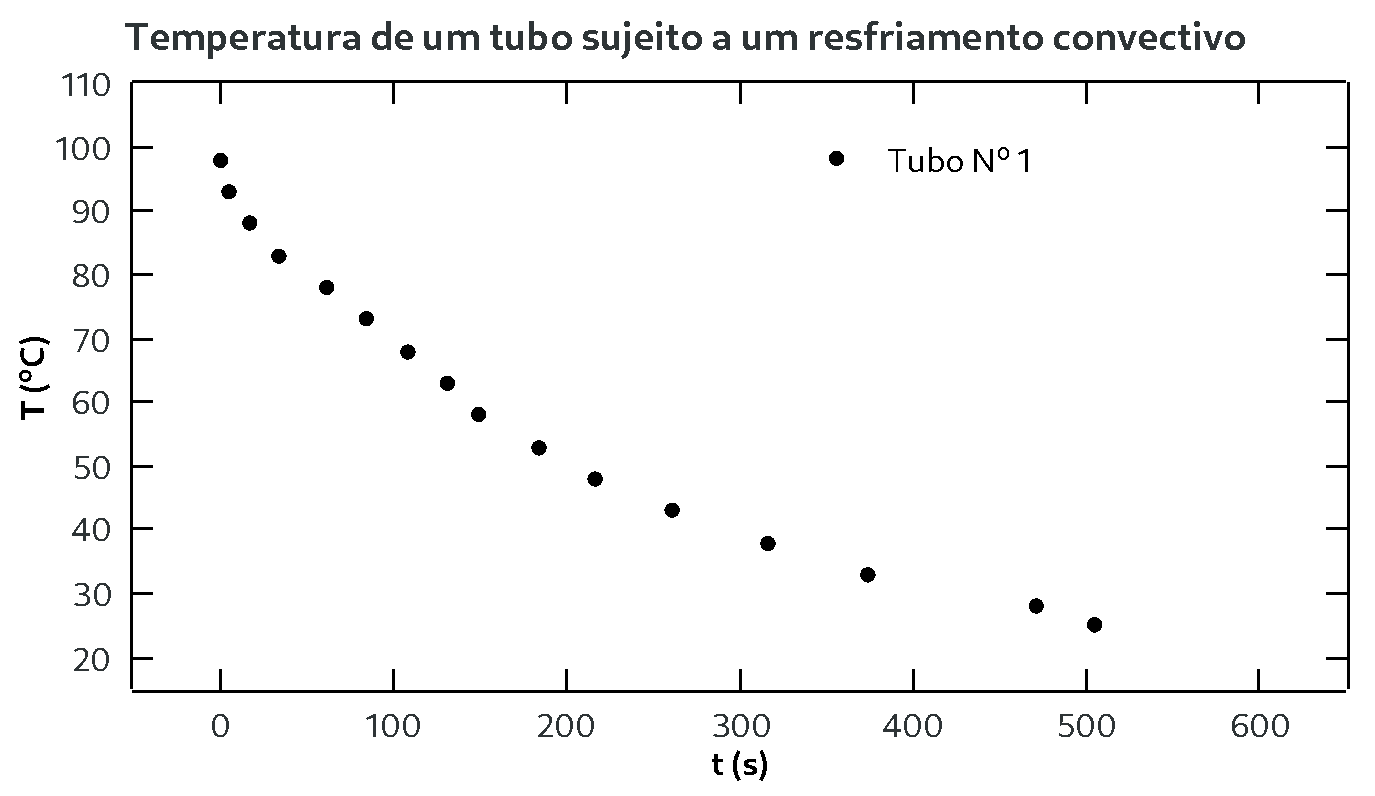
\includegraphics[width=\linewidth]{Graphics/SciDavis/ResultadoSciDavis1.pdf}
\caption{Reprodução da Figura~\ref{Fig:GraficoResfriamento} usando o \emph{SciDavis} usando somente um dos conjuntos de dados. Note que as características da escala correspondem aos da Figura~\ref{Fig:GraficoResfriamento}.\label{Fig:ResultadoSciDavis1}}
\end{figure*}

\pagebreak
%%%%%%%%%%%%%%%%%%%%%%%%%%%%%%%%%%%%%%%%%%%%%%%%%%%%%%%%%%%%%%%%%%%%%%%%
\paragraph{Fazendo gráficos para dois conjuntos independentes de dados:}
%%%%%%%%%%%%%%%%%%%%%%%%%%%%%%%%%%%%%%%%%%%%%%%%%%%%%%%%%%%%%%%%%%%%%%%%

Se os conjuntos de dados não tiverem uma coluna de abscissas em comum, devemos
\begin{enumerate}
    \item Seguir o procedimento para fazer um gráfico para um conjunto de dados, como descrito acima;
    \item em seguida, devemos criar/importar uma nova tabela, selecionar os novos dados, selecionar o gráfico atual e usar o menu `\textsf{Graph > Add/Remove curves}'. Devemos então selecionar o estilo da curva como Scatter selecionar a tabela adequada em `\textsf{Available data}' e clicar na flecha para que a curva seja adicionada a `\textsf{Graph contents}'.\footnote{Note que os nomes em `\textsf{Available data}' são na forma \textsf{TableX\_YYY}, onde \textsf{X} é um número e \textsf{YYY} se refere à coluna que contém as ordenadas; subentende-se automaticamente que a primeira coluna da tabela contém as abscissas daquele conjunto de dados.}
\end{enumerate}

Adicionando mais uma tabela com os dados do Tubo N\textordmasculine~2 da Tabela~\ref{Tab:TabelaDadosResfriamento}, podemos inserir uma nova curva no gráfico da Figura~\ref{Fig:ResultadoSciDavis1}. Fazendo isso, obtemos como resultado o gráfico mostrado na Figura~\ref{Fig:ResultadoSciDavis2}.

\begin{figure*}
\centering
%\forcerectofloat
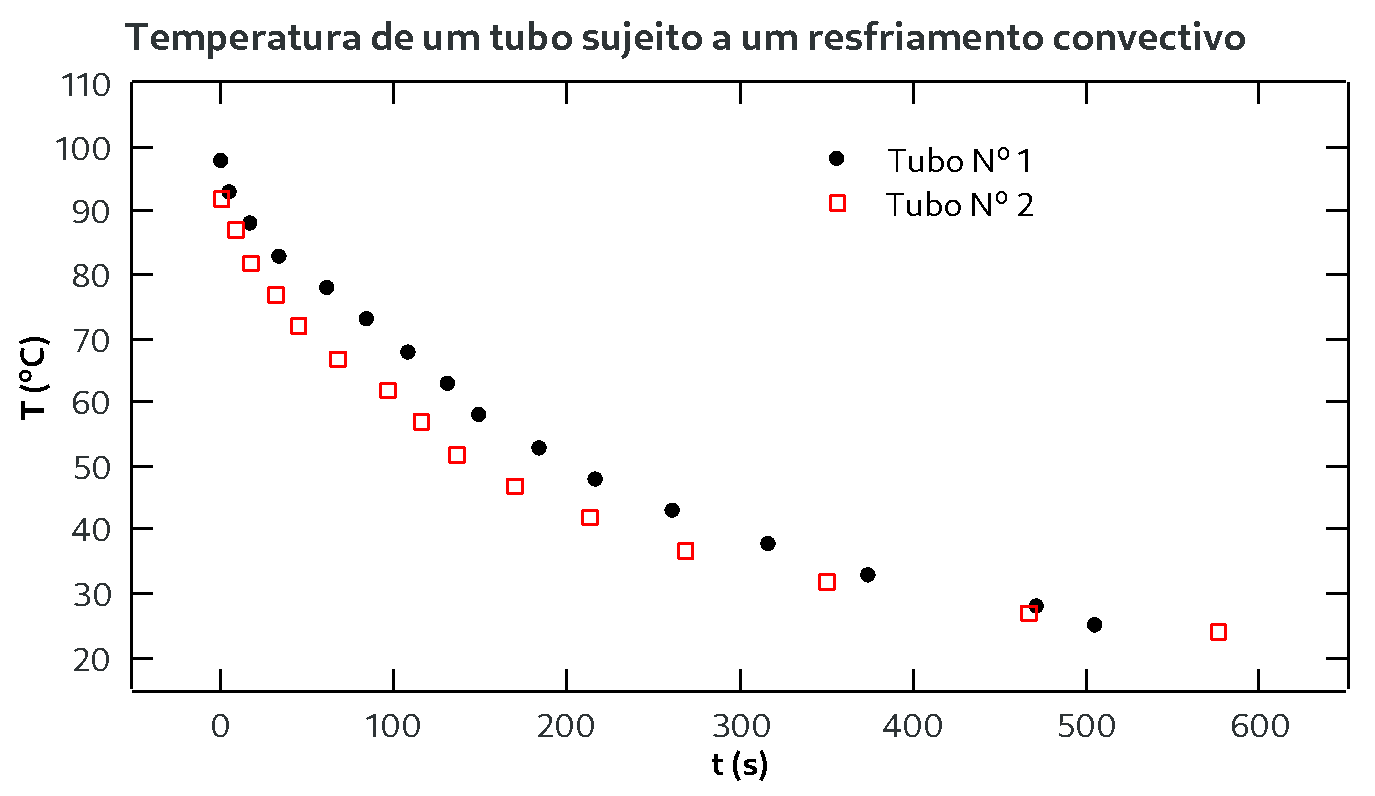
\includegraphics[width=\linewidth]{Graphics/SciDavis/ResultadoSciDavis2.pdf}
\caption{Adicionando os dados relativos ao Tubo N\textordmasculine~2 da Tabela~\ref{Tab:TabelaDadosResfriamento} ao gráfico da Figura~\ref{Fig:ResultadoSciDavis1}, reproduzimos o gráfico da Figura~\ref{Fig:GraficoResfriamento}.\label{Fig:ResultadoSciDavis2}}
\end{figure*}

%%%%%%%%%%%%%%%%%%%%%%%%%%%%%%%%%%%%%%%%%%%%%%%%%%%%%%%%%%%%%%%%%%%%%%%%%%%%%%%%%
\paragraph{Fazendo gráficos para dois conjuntos de dados com abscissas em comum:}
%%%%%%%%%%%%%%%%%%%%%%%%%%%%%%%%%%%%%%%%%%%%%%%%%%%%%%%%%%%%%%%%%%%%%%%%%%%%%%%%%

Para o caso de termos conjuntos de dados em que as abscissas são comuns a mais que um conjunto de ordenadas, a elaboração de um gráfico com múltiplas curvas é mais simples pois podemos armazená-los em uma mesma tabela. Nesse caso, devemos
\begin{enumerate}
	\item inserir os dados em uma tabela ou os importar;
	\item selecionar todas as colunas de dados a serem representadas graficamente; 
	\item selecionar `\textsf{Plot > Scatter}' (no menu principal ou no de contexto).
\end{enumerate}
%
Note que o software assume automaticamente que a primeira coluna é a das abscissas e as demais são as das ordenadas, cada coluna representanto as ordenadas de um conjunto de dados.






\chapter{Software para análise de dados}
\label{Chap:SoftwareDados}

\begin{fullwidth}
{\it
Descrição aqui. Não sei qual é a melhor ordem, se for colocar antes de Regressão, vai ter aqui só a parte de gráficos e será necessário falar que vamos ver em outros capítulos como fazer outras coisas usando o software.
}
\end{fullwidth}

\input{Chapters/Regressao}

\part{Experimentos}
\addtocontents{toc}{\protect\setcounter{tocdepth}{0}}
 
%\input{Experiments/Exp_Modelo}
\input{Experiments/Exp_Medidas}
\input{Experiments/Exp_MRU_MRUV}
%\input{Experiments/Exp_Lancamento_obliquo}
\input{Experiments/Exp_Lei_de_Hooke}
\input{Experiments/Exp_Leis_de_Newton}
\input{Experiments/Exp_Arrasto}
\input{Experiments/Exp_Atrito}
\input{Experiments/Exp_Energia}
\input{Experiments/Exp_Elasticidade}
\input{Experiments/Exp_Empuxo}
\input{Experiments/Exp_Oscilacoes}
%\input{Experiments/Exp_Pendulo_Fisico}
\input{Experiments/Exp_Ondas_Estacionarias}

\printbibliography
\cleardoublepage
\thispagestyle{empty}
\begin{figure*}
\centering
\includegraphics[width = 0.5\linewidth]{Ilustrations/Massa-Mola.png}
\end{figure*}
\vfill
\begin{fullwidth}
\begin{center}\sc
Elaborado usando \LaTeX \\
documentclass: tufte-book \\
imagens tratadas usando Gimp \\
Figuras elaboradas usando tikz
\end{center}
\end{fullwidth}
\end{document}
